\documentclass{article}
\usepackage[paperwidth=20cm, paperheight=4cm, margin = 0cm, top=0.5cm]{geometry}
\usepackage{amsmath}


\usepackage{pgf}
\usepackage{tikz}

\usetikzlibrary{positioning, calc}
\usetikzlibrary{arrows,automata}

\tikzstyle{source}  = [draw,circle,fill=black,thick,inner sep=0mm,minimum size=2mm]

\renewcommand{\vec}[1]{\boldsymbol{#1}}

\begin{document}
\begin{center}
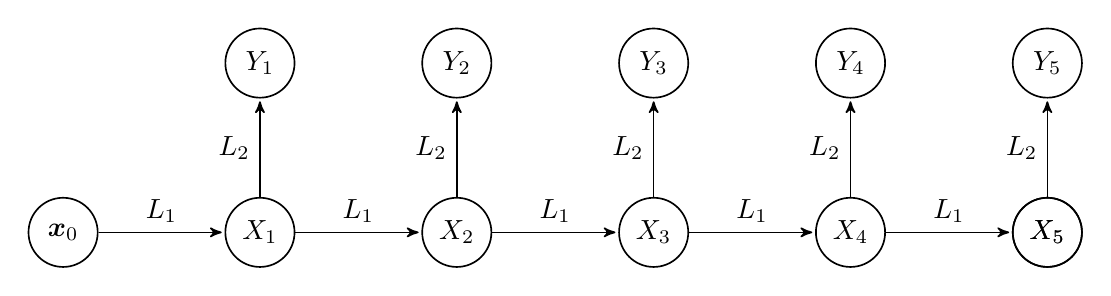
\begin{tikzpicture}[->,>=stealth',shorten >=1pt,auto,node distance=2.5cm,semithick]
                    
\node[state](X0)               {$\vec{x}_0$}; 
\node[state] (X1) [right of=X0] {$X_1$}; 
\node[state] (X2) [right of=X1] {$X_2$};                   
\node[state] (X3) [right of=X2] {$X_3$};                   
\node[state] (X4) [right of=X3] {$X_4$};                   
\node[state] (X5) [right of=X4] {$X_5$};                   
\node[state] (X5) [right of=X4] {$X_5$};                   

\node[state] (Y1) [above = 1.25cm of X1] {$Y_1$}; 
\node[state] (Y2) [right of=Y1] {$Y_2$}; 
\node[state] (Y3) [right of=Y2] {$Y_3$}; 
\node[state] (Y4) [right of=Y3] {$Y_4$}; 
\node[state] (Y5) [right of=Y4] {$Y_5$}; 
	
\path
    (X0) edge node {$L_1$}        (X1)  
	(X1) edge node {$L_1$} (X2)
	(X2) edge node {$L_1$} (X3)
	(X3) edge node {$L_1$} (X4)
	(X4) edge node {$L_1$} (X5);
\path	
	(X1) edge node {$L_2$} (Y1)
	(X2) edge node {$L_2$} (Y2)
	(X3) edge node {$L_2$} (Y3)
	(X4) edge node {$L_2$} (Y4)
	(X5) edge node {$L_2$} (Y5);
\end{tikzpicture}
\end{center}

\end{document}
